% Q16: source PDF p2; hidden AD, DC, DD' and EC dashed.
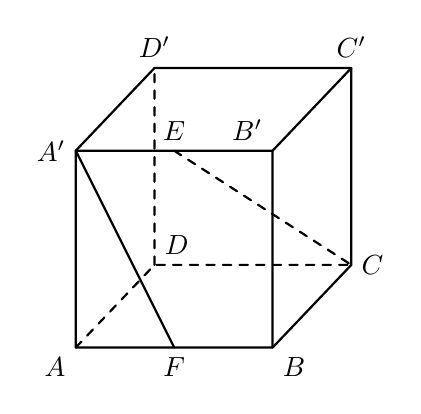
\begin{tikzpicture}[line cap=round,line join=round,thick]
\coordinate (A) at (0,0); \coordinate (B) at (2.5,0);
\coordinate (C) at (3.5,1.05); \coordinate (D) at (1,1.05);
\coordinate (Ap) at (0,2.5); \coordinate (Bp) at (2.5,2.5);
\coordinate (Cp) at (3.5,3.55); \coordinate (Dp) at (1,3.55);
\coordinate (E) at (1.25,2.5); \coordinate (F) at (1.25,0);
\draw[dashed] (A)--(D)--(C) (D)--(Dp) (E)--(C);
\draw (A)--(B)--(C)--(Cp)--(Dp)--(Ap)--cycle;
\draw (Ap)--(Bp)--(Cp) (B)--(Bp) (Ap)--(F);
\node[below left] at (A) {$A$}; \node[below right] at (B) {$B$};
\node[right] at (C) {$C$}; \node[above right] at (D) {$D$};
\node[left] at (Ap) {$A'$}; \node[above left] at (Bp) {$B'$};
\node[above] at (Cp) {$C'$}; \node[above] at (Dp) {$D'$};
\node[above] at (E) {$E$}; \node[below] at (F) {$F$};
\end{tikzpicture}
